\documentclass[xcolor=dvipsnames]{beamer}
%\documentclass[handout,xcolor=dvipsnames,pdftex,hyperref={colorlinks=false}]{beamer}

\usepackage{xcolor}
\usepackage{graphicx}
\graphicspath{{figures/}{.}}
\usepackage{hyperref}
\usepackage{amsmath,amssymb,amsfonts,bm}
\usepackage{colortbl}
\usepackage[english]{babel}
\usepackage{multirow}
\usepackage{booktabs}
\usepackage{array}
\usepackage{tikz}
\usetikzlibrary{arrows.meta, positioning}

\usetheme{Warsaw}
\usepackage{helvet}
\definecolor{someblue}{rgb}{0,.1,0.8}

\renewcommand{\epsilon}{\varepsilon}
\newcommand\E{\mathbb{E}}
\newcommand{\bs}{\boldsymbol}
\newcommand{\mb}{\mathbf}
\renewcommand{\b}{\ensuremath{\bs{\beta}}}
\newcommand{\Z}{\ensuremath{\mb{Z}}}
\newcommand{\X}{\ensuremath{\mb{X}}}
\newcommand{\Y}{\ensuremath{\mb{Y}}}
\newcommand{\D}{\ensuremath{\mb{D}}}

\newcommand{\indep}{{\bot\negthickspace\negthickspace\bot}}

\newtheorem{assumption}{Assumption}
\newtheorem{iass}{Identification Assumption}
\newtheorem{ires}{Identification Result}
\newtheorem{estm}{Estimand}
\newtheorem{esti}{Estimator}

\title[]{Instrumental Variables}
\subtitle[ ]{PS200C, Spring 2026}
\author[Hazlett]{Chad Hazlett}
\institute[UCLA]{UCLA\\[1ex]
  \texttt{chazlett@ucla.edu}
}
\date{}

\definecolor{dgreen}{rgb}{0,.6,0.8}
\useoutertheme{infolines}

\begin{document}

\begin{frame}
  \titlepage
\end{frame}

%================================================================
% 1. Where we are
%================================================================
\begin{frame}{Where we are}
\begin{itemize}
\item<1-> For SOO, we leaned on \textcolor{Blue}{conditional ignorability}: find an $X$ that closes all back-doors, then adjust for it.
\medskip
\item For DID, we traded ignorability in levels for ignorability in trends (\textcolor{Blue}{parallel-trends})
\medskip
\item Today, a different bargain: Try to find an ``encouragement'' to treatment, which only matters through treatment, identifying an effect in a sub-group.
\end{itemize}
% \bigskip
% \onslide<2->\textcolor{Blue}{The trade:} pick a variable $Z$ that randomly nudges $D$ but is otherwise irrelevant for $Y$. Use only the $D$-variation that $Z$ generates.
\end{frame}

%================================================================
% 2. The encouragement design intuition (compressed)
%================================================================
\begin{frame}{The intuition: a randomized encouragement}
\onslide<1-> Suppose we can't randomize \textit{pizza} (IRB won't allow withholding pizza), but we \textit{can} randomize a \textit{gift card} for pizza.\\
\bigskip
\onslide<2-> Half the sample gets a card; we observe who actually eats pizza, then measure happiness.\\
\bigskip
\onslide<3-> \textcolor{Blue}{Good news:} we have an experiment with respect to the card.
\begin{itemize}
\item<4-> $\E[\text{happy} \mid \text{card}] - \E[\text{happy} \mid \text{no card}]$ is identified.\\
This is the \textcolor{Blue}{intent-to-treat (ITT)} or \textcolor{Blue}{reduced form} effect of the card.
\item<5-> \textcolor{Red}{But it isn't the effect of pizza.} How do we get back to that?
\end{itemize}
\end{frame}

\begin{frame}{Backing it out: four kinds of people}
\onslide<1-> Imagine four groups defined by how they respond to the encouragement:
\small
\begin{itemize}
\item<2-> \textit{Never-takers}: don't eat pizza either way. \textcolor{Blue}{Card has no effect on their pizza intake $\Rightarrow$ no effect on their happiness.}
\smallskip
\item<3-> \textit{Always-takers}: eat pizza either way. \textcolor{Blue}{Same: card doesn't change anything for them.}
\smallskip
\item<4-> \textit{Compliers}: eat pizza \textit{iff} they get the card. \textcolor{Blue}{For them, card means pizza, no card means no pizza: effect of card (ITT) is effect of pizza.}
\smallskip
\item<5-> \textit{Defiers}: eat pizza \textit{iff} they don't get the card. \textcolor{Red}{We assume away.}
\end{itemize}
\bigskip
\onslide<6-> \normalsize \textcolor{Blue}{Punchline:} the ITT over everyone will be an average over these and so will be a \textit{watered-down} version of the pizza effect. Specifically,
\end{frame}

\begin{frame}{Backing it out: the algebra}
\small
\onslide<1-> Averaging the ITT over the four types:\\
\footnotesize
\begin{align*}
\text{ITT} \;=\; & \underbrace{(\text{ITT}\mid \text{never-taker})}_{=0}\cdot \Pr(\text{never-taker}) \\
&+\; \underbrace{(\text{ITT}\mid \text{always-taker})}_{=0}\cdot \Pr(\text{always-taker}) \\
&+\; \textcolor{Blue}{(\text{ITT}\mid \text{complier})\cdot \Pr(\text{complier})} \\
&+\; \underbrace{(\text{ITT}\mid \text{defier})}_{=0,\;\text{by assumption}}\cdot \Pr(\text{defier}) \\[2pt]
\Rightarrow\quad \text{ITT}\mid\text{complier} \;=\;& \frac{\text{ITT}}{\Pr(\text{complier})}
\end{align*}
\medskip
\onslide<2-> \normalsize \textcolor{Blue}{So we can recover an ITT-for-compliers.} \\
\medskip
\onslide<3-> And for compliers, the ITT is the ATE.
\end{frame}

\begin{frame}{From ITT-on-compliers to LATE}
\small
\onslide<1-> One more thing you need to know: $\Pr(\text{complier})$ is the ``first stage'' effect:\\

\bigskip

$\Pr(\text{complier}) = \E[D_1 - D_0] = \E[D|Z=1]-\E[D|Z=0]$ (by ignorability of $Z$), which equals the proportion of compliers (if no defiers).

\bigskip

\onslide<4-> \small Putting it together: We call the ATE among the compliers the ``local average treatment effect'' (LATE):

\begin{center}
\textcolor{Blue}{$\displaystyle \text{LATE} \;=\; \frac{\text{ITT}}{\text{Pr(complier)}}\; = \; \frac{\E[Y\mid Z=1]-\E[Y\mid Z=0]}{\E[D\mid Z=1]-\E[D\mid Z=0]}$}
\end{center}
\end{frame}

%================================================================
% Identification (3)

%================================================================
\begin{frame}{Formalizing this potential-outcomes machinery}
\small
Let $Z_i\in\{0,1\}$ be the encouragement (\textcolor{Blue}{instrument}) and $D_i\in\{0,1\}$ the treatment.\\

\bigskip

\textbf{Potential treatments.} $D_{1i}$, $D_{0i}$: would you take the treatment if encouraged ($Z=1$) or not ($Z=0$).
\smallskip
We see $D_i = Z_i D_{1i} + (1-Z_i) D_{0i}$.
\medskip

\textbf{Four principal strata}, defined by $(D_{0i},D_{1i})$:
\begin{center}
\begin{tabular}{l|cc}
& $D_{0i}=0$ & $D_{0i}=1$\\\hline
$D_{1i}=0$ & never-taker & \textcolor{Red}{defier}\\
$D_{1i}=1$ & \textcolor{Blue}{complier} & always-taker\\
\end{tabular}
\end{center}

\medskip
\textbf{Monotonicity} $\;D_{1i}\geq D_{0i}$ for all $i$ rules out the red cell.
\end{frame}

% \begin{frame}{LATE: the assumptions}
% \begin{iass}
% \begin{enumerate}
% \item \textbf{Relevance / first stage:} $\Pr(D_{1}=1)\neq \Pr(D_{0}=1)$\;---\; $Z$ moves $D$.
% \medskip

% \item \textbf{Exclusion:} $Y(d,z) = Y_d$\;---\; $Z$ affects $Y$ only through $D$.

% \medskip

% \item \textbf{Ignorability of $Z$:} $\;\{Y(d), D(z)\} \indep Z$ for all $d,z$\;---\; $Z$ random.

% \medskip

% \item \textbf{Monotonicity:} $D_{1i}\geq D_{0i}$\;---\; no defiers.
% \end{enumerate}
% \end{iass}
% % \medskip
% % \footnotesize
% % \onslide<2->{Note the order: exclusion first lets us collapse the four potential outcomes $Y(d,z)$ to two, $Y_d$. Then ignorability is just w.r.t.\ those.}
% % \bigskip
% % \onslide<3->{\small Under (1)--(4), the \textcolor{Blue}{LATE} (effect on compliers) is identified by the Wald ratio.}
% \end{frame}

% \begin{frame}{Identification result}
% \begin{ires}
% \footnotesize
% Under the four assumptions:
% \begin{align*}
% \E[Y_1-Y_0 \mid \text{complier}] \;=\; \frac{\E[Y\mid Z=1]-\E[Y\mid Z=0]}{\E[D\mid Z=1]-\E[D\mid Z=0]}
% \;=\; \frac{\text{ITT (effect of Z on Y)}}{\text{first stage (effect of Z on D)}}
% \end{align*}
% \end{ires}
% \medskip
% \onslide<2->{\small \textcolor{Blue}{Read this carefully.}}
% \footnotesize
% \begin{itemize}
% \item<3-> The numerator and denominator are \textit{both} just experimental quantities --- effects of a randomly assigned $Z$ on $Y$ and on $D$.
% \smallskip
% \item<4-> The ratio recovers a treatment effect, but only \textit{for compliers}. Different instrument $\Rightarrow$ different complier group $\Rightarrow$ a different LATE.
% \smallskip
% \item<5-> Proof sketch in the appendix.
% \end{itemize}
% \end{frame}

 \begin{frame}{The assumptions}
 \small

 \textbf{1. Exclusion}: $Y(d,z) = Y_d$: $Z$ affects $Y$ only through $D$. 
 \begin{itemize}
 \item \textcolor{Red}{Not implied} by $Z$ being random: $Z$ can be random but \textit{still} affect $Y$ through some channel other than $D$.
 \item Not testable though sometimes falsifiable.  
 \end{itemize} 
 \medskip

 \textbf{2. Ignorability} of $Z$: $\{Y(d), D(z)\} \indep Z$ for all $d,z$. 
 \begin{itemize}
 \item Ideally $Z$ is literally randomized, or pseudo-randomized (some ``shock'')
 \end{itemize} 
 \medskip

 \textbf{3. First stage / relevance}:  $\Pr(D_{1}=1)\neq \Pr(D_{0}=1)$\;---\; i.e. there are some compliers. Testable: regress $D$ on $Z$.  \\

%  \begin{itemize}
%   \item  \textcolor{Red}{Weak instruments} are bad: tiny denominator $\Rightarrow$ huge variance, and small bias gets blown up.
%   \item Rule of thumb $F>10$ (better: Anderson--Rubin CIs).
%  \end{itemize}
 \medskip
 \textbf{4. Monotonicity}: $D_{1i}\geq D_{0i}$\;---\; no defiers. Not testable, but often qualitatively defensible (e.g.\ a lottery winner is no \textit{less} likely to enroll).
 \end{frame}

%================================================================
% IV DAG
%================================================================
\begin{frame}{The IV DAG}
\begin{center}
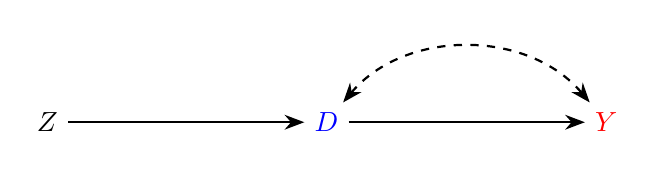
\begin{tikzpicture}[->, >={Stealth[length=2.5mm]}, thick, node distance=3cm]
    \node (Z) {$Z$};
    \node[right=of Z] (D) {\textcolor{blue}{$D$}};
    \node[right=of D] (Y) {\textcolor{red}{$Y$}};
    \draw (Z) -- (D);
    \draw (D) -- (Y);
    \draw[dashed, <->] (D) to[bend left=50] (Y);
\end{tikzpicture}
\end{center}
\onslide<1-> This would be good.
\small
\begin{itemize}
  \item Unobserved confounders of $D$ and $Y$ -- no problem!
  \item But what's important is what's not on here...
\end{itemize}
\medskip
\end{frame}

\begin{frame}{The IV DAG: edges that should \textit{not} be there}
\begin{center}
\begin{tikzpicture}[->, >={Stealth[length=2.5mm]}, thick, node distance=3cm]
    \node (Z) {$Z$};
    \node[right=of Z] (D) {\textcolor{blue}{$D$}};
    \node[right=of D] (Y) {\textcolor{red}{$Y$}};
    \draw (Z) -- (D);
    \draw (D) -- (Y);
    \draw[dashed, <->] (D) to[bend left=50] (Y);
    % Violations
    \draw[dashed, <->, red, thick] (Z) to[bend left=80] (Y);
    \draw[dashed, ->,  red, thick] (Z) to[bend right=40] (Y);
\end{tikzpicture}
\end{center}
\footnotesize
\textcolor{Red}{Red edges} are the ones an IV story \textit{must} rule out:
\begin{itemize}
\item Top: $Z \leftrightarrow Y$: \textit{any} unobserved factor associated with both $Z$ and $Y$. \textcolor{Red}{Violates ignorability of $Z$.}
\item Bottom: $Z \to Y$: a direct path from $Z$ to $Y$ not via $D$. \textcolor{Red}{Violates exclusion.}
\end{itemize}
\end{frame}

%================================================================
% Estimation (2)
%================================================================
\begin{frame}{Estimation: Wald and 2SLS}
\small
\textbf{Wald estimator} (sample analog of the ratio):
\[
\hat\beta_{\text{Wald}} \;=\; \frac{\bar Y_{Z=1} - \bar Y_{Z=0}}{\bar D_{Z=1} - \bar D_{Z=0}}
\]
\medskip
\textbf{Two-stage least squares (2SLS):}
\begin{enumerate}
\item First stage: $D_i = \pi_0 + \pi Z_i + \eta_i$. Compute $\hat D_i$.
\item Second stage: $Y_i = \beta_0 + \beta\, \hat D_i + \varepsilon_i$.
\end{enumerate}
\bigskip
With one binary $Z$ and one binary $D$, $\hat\beta_{\text{2SLS}} = \hat\beta_{\text{Wald}}$.\\
\bigskip
\onslide<2-> In practice: for $\X=[1\ D]$, $\hat{\beta}_{IV} = (Z^{\top}\X)^{-1} Z^{\top}Y$.\\
\begin{itemize}
\item \textbf{In R:} \texttt{ivreg(Y $\sim$ D | Z)} from the \texttt{AER} package.
\end{itemize}
% \medskip
% \onslide<3-> \textcolor{Red}{Don't run the two stages by hand} --- you'll get the wrong SEs.
\end{frame}

\begin{frame}{Estimation: covariates and weak instruments}
\small
\textbf{Adding covariates} when ignorability/exclusion only hold conditional on $X$:
\begin{itemize}
\item Add $X$ to \textit{both} stages.
\item With heterogeneous effects, this no longer cleanly identifies a LATE; the complier set varies with $X$. %Most applied work either (a) accepts a constant-effects approximation or (b) uses $\kappa$-weighting (Abadie 2003) to recover an effect on compliers.
\end{itemize}
\bigskip

\textbf{Weak instrument diagnostics:}
\begin{itemize}
\item First-stage $F$-statistic; rule of thumb $F>10$.
\item Better: \textcolor{Blue}{Anderson--Rubin} confidence intervals --- valid even when the instrument is weak.
\end{itemize}
\end{frame}

%================================================================
% RCT with non-compliance --- the cleanest IV
%================================================================
\begin{frame}{The ideal use-case: RCTs with non-compliance}
\onslide<1-> Suppose you run a randomized trial, \\
\small
\begin{itemize}
\item Assigned \textcolor{Blue}{treatment} ($Z$), but $D$ means actual take-up.
\item Could be one-way or two-way non-compliance.
\end{itemize}
\bigskip

\onslide<2-> You might estimate the ITT, i.e. the effect of \textit{being assigned} to treatment. 
\begin{itemize}
\item<3-> Easy, unbiased, but \textcolor{Red}{understates the effect of the treatment itself}.
\end{itemize}

\bigskip
\onslide<3-> \textbf{The IV ``correction''}: divide that ITT by compliance rate to get back the ``undiluted'' effect of actually \textit{taking} the treatment, but only for \textit{compliers}.
\medskip
\begin{itemize}\footnotesize
\item \textcolor{Blue}{Ignorability} of $Z$: holds \textit{by design} (the experimenter randomized).
\item \textcolor{Blue}{Exclusion}: could still be violated but could be defensible -- some $Y$s are hard to move without special treatment.
\item \textcolor{Blue}{Monotonicity}: usually defensible.
\end{itemize}

\medskip
\onslide<5-> This is standard fare in many RCTs and field experiments.
\end{frame}

%================================================================
% Famous designs (2 frames)
%================================================================
\begin{frame}{Three famous IV Examples}
\vspace{-0.05in}
\scriptsize
\begin{center}
\renewcommand{\arraystretch}{1.25}
\begin{tabular}{p{1.15in} p{1.35in} p{0.85in} p{0.85in} p{1.45in}}
\toprule
\textbf{Setup} & \textbf{Instrument $Z$} & \textbf{Treatment $D$} & \textbf{Outcome $Y$} & \textbf{Who are the compliers?}\\
\midrule
\textbf{Acemoglu, Johnson \& Robinson (2001)}\newline\textit{settler mortality} & European settler mortality, c.\ 1500--1900 & quality of institutions today & log GDP per capita & countries whose colonial institutions were shaped by how habitable Europeans found them\\[2pt]
\textbf{Angrist \& Krueger (1991)}\newline\textit{quarter of birth} & quarter of birth (Q1 vs.\ Q3/Q4) & years of schooling & log earnings & kids on the margin of compulsory-schooling-law cutoffs (drop out as soon as legal)\\[2pt]
\textbf{Miguel, Satyanath \& Sergenti (2004)}\newline\textit{rainfall and conflict} & year-on-year rainfall growth & income / GDP growth & civil conflict onset & rainfall-sensitive (rural, ag) economies whose income tracks rainfall\\
\bottomrule
\end{tabular}
\end{center}
\medskip
\small
\onslide<2-> Who are the compliers in each? \\
\onslide<3-> Let's worry about ignorability in each. \\
\onslide<4-> Let's worry about exclusion in each.
\end{frame}

% \begin{frame}{What we'd worry about}
% \vspace{-0.05in}
% \scriptsize
% \begin{center}
% \renewcommand{\arraystretch}{1.3}
% \begin{tabular}{p{.5in} p{2.4in} p{2.4in}}
% \toprule
% \textbf{Setup} & \textbf{Ignorability worry (is $Z$ really as-if random?)} & \textbf{Exclusion worry (does $Z$ affect $Y$ \textit{only} through $D$?)}\\
% \midrule
% \textbf{AJR}\newline\textit{settler mortality} & where Europeans went and how they measured mortality is not random; mortality data quality varies systematically & disease environment \textit{persists}: malaria etc.\ may directly suppress productivity today, not only via institutions\\[2pt]
% \textbf{AK91}\newline\textit{quarter of birth} & truly random (calendar) & season of birth correlates with maternal nutrition, schooling cohort effects, age-at-test-cutoffs --- all could affect earnings outside of years-of-schooling\\[2pt]
% \textbf{Miguel et al.}\newline\textit{rainfall} & weather is largely exogenous, but predictable patterns shape settlement and agriculture & rainfall affects conflict directly: mobility, troop logistics, mood/grievance, beyond income\\
% \bottomrule
% \end{tabular}
% \end{center}
% \medskip
% \onslide<2->{\footnotesize \textcolor{Red}{Random $Z$ is not enough.} Always force yourself to write down the channels by which $Z$ could touch $Y$ \textit{without going through $D$}.}
% \end{frame}

%================================================================
% Running application: Angrist 1990 (3 frames)
%================================================================
\begin{frame}{Application: Vietnam draft lottery (Angrist 1990)}
\small
\onslide<1-> \textbf{Question:} What is the causal effect of military service on later civilian earnings? \\
\medskip

\onslide<2-> \textbf{The naive comparison} (veterans vs.\ non-veterans) is hopeless: who served depends on health, education, wealth, region, family, motivation \ldots\ which may predict earnings. \\
\medskip

\onslide<3-> \textbf{Angrist's idea:} use the \textcolor{Blue}{Vietnam-era draft lottery} (1969--72). Each birthday was randomly assigned a number 1--365; the Selective Service then announced a yearly cutoff, and men with numbers \textit{below} the cutoff were called for induction.
\smallskip
\begin{itemize}
\item $Z = 1$ \textit{draft-eligible}: number below the cutoff $\Rightarrow$ called for induction
\item $D = 1$: actually served in the military
\item $Y$: civilian earnings, 1981--84
\end{itemize}
\medskip

\onslide<4-> \textcolor{Blue}{Critical:} \textit{$Z\neq D$}. Among the called ($Z=1$), only $\sim$35\% served (deferments, failed physicals). Among the not-called ($Z=0$), $\sim$19\% still served (volunteers). First stage $\approx 0.16$.

\end{frame}

\begin{frame}{Wald estimates from Angrist (1990): white men, 1950 cohort}
\small

\begin{center}
\renewcommand{\arraystretch}{1.4}
\begin{tabular}{l r}
\toprule
\textcolor{Blue}{ITT} \quad ($\bar Y^e - \bar Y^n$, 1981 FICA earnings)             & $-\$435.8$ \;\; (s.e.\ 210.5) \\
\textcolor{Blue}{First stage} \quad ($\hat p^e - \hat p^n$, veteran rate)           & $0.159$ \;\; (s.e.\ 0.040) \\
\midrule
\textcolor{Blue}{Wald} \;$=$\; ITT $/$ first stage    & $\dfrac{-435.8}{0.159} \;\approx\; -\$2{,}741$ \;\; (s.e.\ $\approx\!\$1{,}335$) \\
\bottomrule
\end{tabular}

\smallskip
{\scriptsize Source: Angrist (1990) Table~3, col.~1.}

\end{center}

\onslide<2-> What's the interpretation of this result?

% \medskip
% \footnotesize
% \textit{First stage:} lottery eligibility raised the veteran rate by $\sim$\textbf{16pp}.\\[2pt]
% \textit{ITT:} eligible cohorts earned $\sim$\textbf{\$436 less} in 1981 FICA earnings.\\[2pt]
% \textit{Wald:} per veteran \textit{induced into service by the lottery}, that's a $\sim$\textbf{\$2{,}740/yr} earnings hit ($\sim$15\% of mean earnings) --- imprecise.
\end{frame}

\begin{frame}{What about the assumptions here?}
\small
\textbf{Ignorability of $Z$?} \onslide<2-> \textcolor{Blue}{Yes by design} --- it's a uniform random number.
\bigskip

\textbf{First stage / relevance?} \onslide<3-> Lottery eligibility raised the probability of service by $\sim$16 percentage points; $F = (0.159/0.040)^2 \approx 16$. Considered okay. 
\bigskip

\textbf{Monotonicity?} \onslide<4-> Hard to imagine someone served \textit{only} because they got a high (safe) lottery number. Defensible.
\bigskip

\textbf{Exclusion restriction?} \onslide<5-> \textcolor{Red}{e.g. College deferments.}
\begin{itemize}
\item Men with low lottery numbers were draft-eligible, had incentive to enroll in college to claim a student deferment.
\item Thus draft-eligible men ended up with \textit{more} schooling
\item ...$Z$ can lead to higher earnings via schooling, not only via service.
\end{itemize} 

\bigskip

\textcolor{Blue}{LATE for whom?} \footnotesize \onslide<6-> Lottery-induced compliers: those who served \textit{because} of their number. Not always-takers (volunteers), not never-takers (medically deferred).
\end{frame}

%================================================================
% Wrap
%================================================================
\begin{frame}{Rules of the game}
\begin{enumerate}
\item Show \textcolor{Blue}{Relevance}: $Z$ moves $D$. \textit{Look at the first stage.}
\medskip
\item \textcolor{Blue}{Ignorability + exclusion}: ignorability is given by random $Z$; still worry about exclusion. \textit{Not verifiable but explain why you believe it. You can show certain (observed) channels can be ruled out.}
\medskip
\item \textcolor{Blue}{Monotonicity}: no defiers. \textit{Often you can argue this on qualitative grounds.}
\medskip
\item \textcolor{Blue}{Interpretation}: LATE for compliers. \textit{Who are the compliers? Are they policy-relevant?}
\end{enumerate}
\end{frame}

% %================================================================
% % Appendix
% %================================================================
% \appendix

% \begin{frame}{Appendix: identification proof}
% \scriptsize
% By exclusion, $Y_i = Y_{0i}+(Y_{1i}-Y_{0i})D_i$. By ignorability of $Z$, $\E[Y\mid Z=z]=\E[Y_0+(Y_1-Y_0)D_z]$. Then
% \begin{multline*}
% \frac{\E[Y\mid Z=1]-\E[Y\mid Z=0]}{\E[D\mid Z=1]-\E[D\mid Z=0]}
% \;=\; \frac{\E[(Y_1-Y_0)(D_1-D_0)]}{\E[D_1-D_0]} \\
% \;=\; \frac{\E[Y_1-Y_0\mid D_1>D_0]\Pr(D_1>D_0) - \E[Y_1-Y_0\mid D_1<D_0]\Pr(D_1<D_0)}{\Pr(D_1>D_0)-\Pr(D_1<D_0)}.
% \end{multline*}
% By monotonicity, $\Pr(D_1<D_0)=0$, so this collapses to $\E[Y_1-Y_0\mid D_1>D_0]$, the LATE. $\square$
% \end{frame}

\end{document}
